\documentclass[runningheads,a4paper]{llncs}

%
\usepackage{amssymb}
\usepackage{amsmath}
\usepackage{url}
\usepackage{graphicx}
\usepackage{multirow}
\usepackage{wrapfig}
\usepackage{hyperref}
\usepackage{color}
\usepackage[font=small,labelfont=bf]{caption}

\newcommand{\rk}[1]{{\color{red}{#1}}}

%
\newcommand{\argmin}[1]{\underset{#1}{\operatorname{arg}\operatorname{min}}\;}
\setlength{\belowcaptionskip}{-15pt}
\setlength{\abovecaptionskip}{-2pt}
%
\mathchardef\mhyphen="2D
\raggedbottom 
%
% Allow easy processing of labeled images in figures
\newcounter{lfigcounter}
\newenvironment{IonTab}{\begin{table}[htb]}{\end{table}}
\newenvironment{IonFig}{\setcounter{lfigcounter}{1}\begin{figure}} {\end{figure}}
\newenvironment{IonFigH}{\setcounter{lfigcounter}{1}\begin{figure}[h]}{\end{figure}}
\newenvironment{IonFigT}{\setcounter{lfigcounter}{1}\begin{figure}[!t]}{\end{figure}}
\newenvironment{IonFigB}{\setcounter{lfigcounter}{1}\begin{figure}[b]}{\end{figure}}
\def\ionbox#1{\makebox[#1]{(\alph{lfigcounter})}\stepcounter{lfigcounter}}
%
\begin{document}

\mainmatter  % start of an individual contribution

% first the title is needed
\title{An Image-based method for phase estimation, gating and temporal super-resolution of \\cardiac ultrasound}

% a short form should be given in case it is too long for the running head
\titlerunning{An Image-based Phase Estimation Method for Cardiac Ultrasound}

% the name(s) of the author(s) follow(s) next
%
% NB: Chinese authors should write their first names(s) in front of
% their surnames. This ensures that the names appear correctly in
% the running heads and the author index.
%

% anonymous stuff
\author{*}
\authorrunning{*}   
\tocauthor{*}
\institute{*}

\maketitle

\begin{abstract}
Ultrasound is emerging as an increasingly effective tool for rapid non-invasive assessment of cardiac structure and function. Knowledge of the phase or location of each video frame within the cardiac and/or respiratory cycles is essential in many applications and is particularly challenging in pre-clinical studies involving small animals with rapid heart and respiration rates. In this paper, we present a novel method for estimation of instantaneous cardiac and respiratory phases directly from cardiac ultrasound videos. The method transforms the complex high-dimensional image sequence into a univariate time series with the same periodicity characteristics, decouples the periodic sources of beating heart and respiratory motion using a trend extraction technique, and estimates the cardiac and respiratory phases using the Hilbert transform. We also present a robust non-parametric regression technique for gating out respiratory frames and a kernel regression model that reconstructs images at any cardiac phase and facilitates temporal super-resolution. We validate our methods using cardiac ultrasound or echocardiography videos and ECG recordings of 6 mice.
%\keywords{Cardiac, Ultrasound, Echocardiography, Phase estimation, Gating, Temporal Super-resolution}
\vspace{-0.3cm}
\end{abstract}
%
\section{Introduction}
\label{sec:intro}
%
Cardiovascular disease is the leading cause of death worldwide and ultrasound is emerging as an increasingly effective tool for rapid non-invasive assessment of cardiac structure and function. Cardiac ultrasound videos consist of two kinds of periodic motion, one corresponding to beating heart motion and the other corresponding to respiratory motion. Knowledge of the phase or location of each video frame within the cardiac and/or respiratory cycles is essential in a variety of applications such as gating \cite{Sundar2009}, quiescence detection~\cite{Wick2013}, 3D reconstruction~\cite{VonBirgelen1997}, and temporal super-resolution~\cite{Cherin2006}. These tasks are particularly challenging in pre-clinical studies involving small animals such as mice that have rapid heart (310-840 BPM) and respiration (80-230 BPM) rates. Typically, the position within cardiac cycle is tracked through ECG data and position within the respiratory cycle is tracked by motion of markers placed on the subject's body \cite{Khamene2004}. 

\vskip0.5ex
\noindent
\textbf{Contributions.} In this paper, we present a novel method that estimates the instantaneous cardiac and respiratory phases directly from the cardiac ultrasound video(Figure~\ref{fig:phase_estimation}). We also present a robust non-parametric regression technique for gating out respiratory frames and a novel kernel regression model for reconstructing images at any cardiac phase to facilitate temporal super-resolution. 

\vskip0.5ex
\noindent
\textbf{Related work.} Previous work on estimation of cardiac and/or respiratory phases directly from ultrasound videos is very limited. In~\cite{Karadayi2006}, the authors compute a signal of the x- or y-coordinate of the center-of-mass of each frame, use bandpass filtering to remove components outside the cardiac frequency range, and apply matched sine/cosine filters to estimate the instantaneous phase. In~\cite{Sundar2009}, the authors compute a signal of phase correlation between consecutive frames and use an approach similar to~\cite{Karadayi2006} to recover the cardiac and respiratory signals. The center-of-mass signals are not reliable and phase correlation finds global translation that does not model beating and out-of-plane heart motion well.

\vspace{-0.3cm}
\section{Method}
\label{sec:method}
\vspace{-0.3cm}
%
In this section, we present the theory underlying the proposed methods.
In Section~\ref{sec:method:phase_estimation}, we describe our method for estimation of instantaneous cardiac and respiratory phases. In Section~\ref{sec:method:gating}, we present a robust method to exclude video frames with significant respiratory motion. In Section~\ref{sec:method:super_resolution}, we present a kernel regression model for reconstructing images at any cardiac phase to facilitate temporal super-resolution.
%
%
\begin{IonFigT}
\centering
%
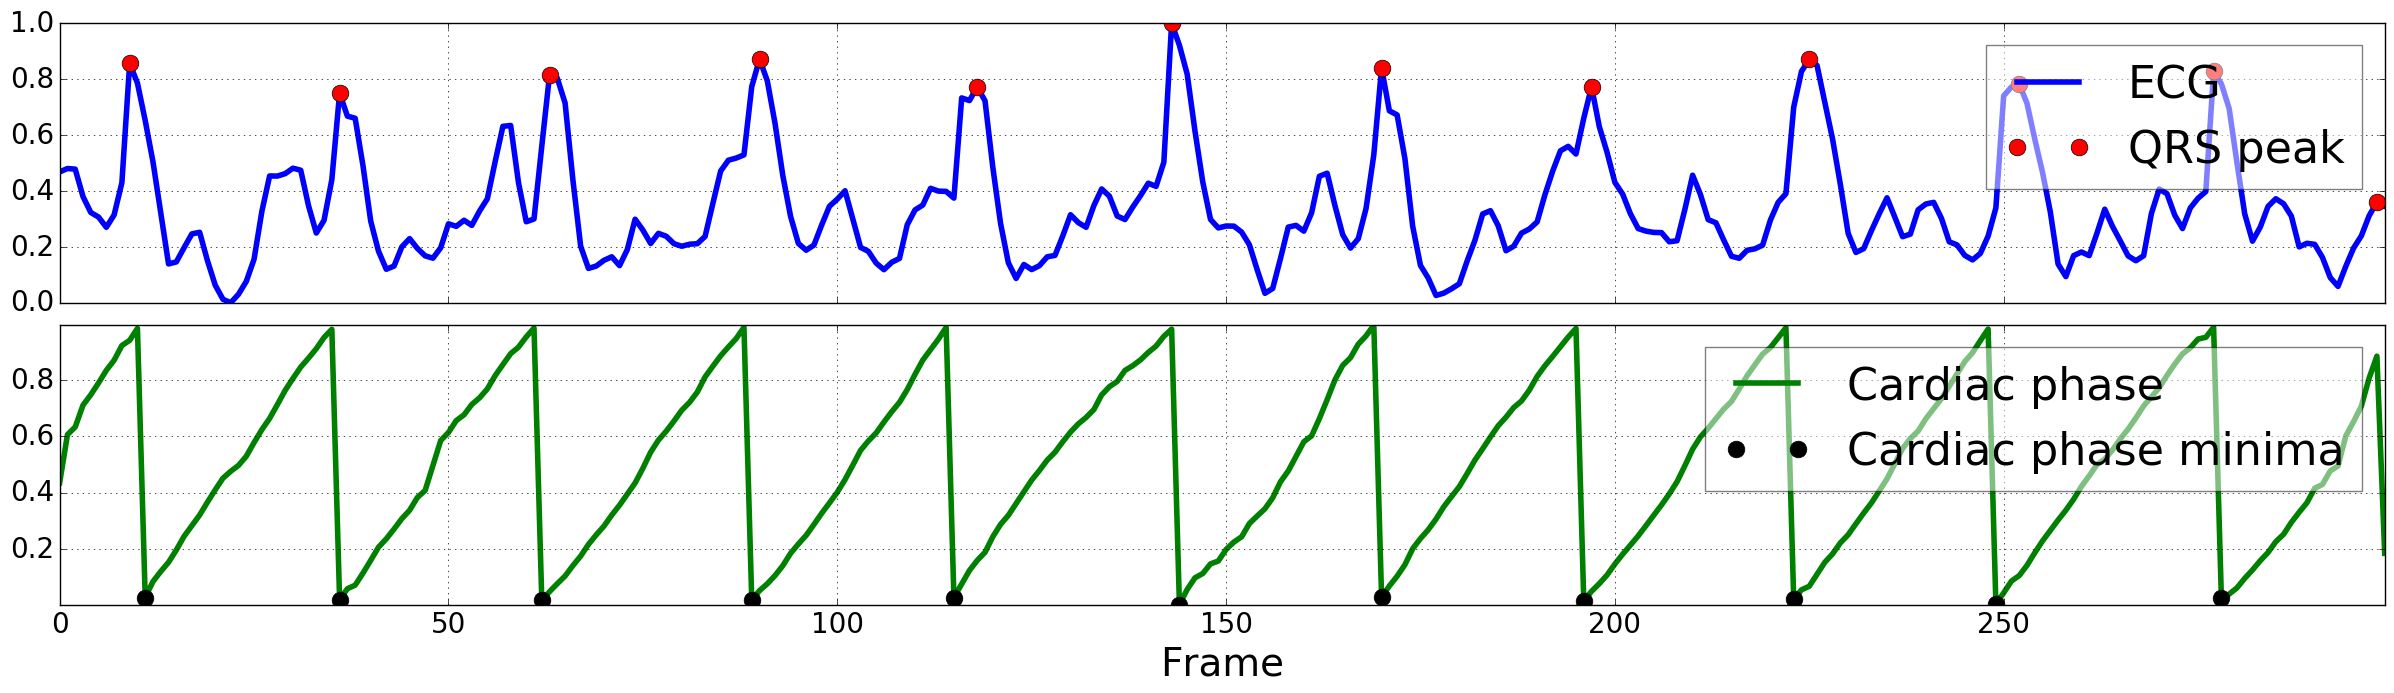
\includegraphics[width=4.25in]{figures/decoded/2015-07-27-10-36-06_2015-07-15-16-56-16_1.raw.bmode/ecg_instaphase_overlay.png}\\
\ionbox{4.25in}\\
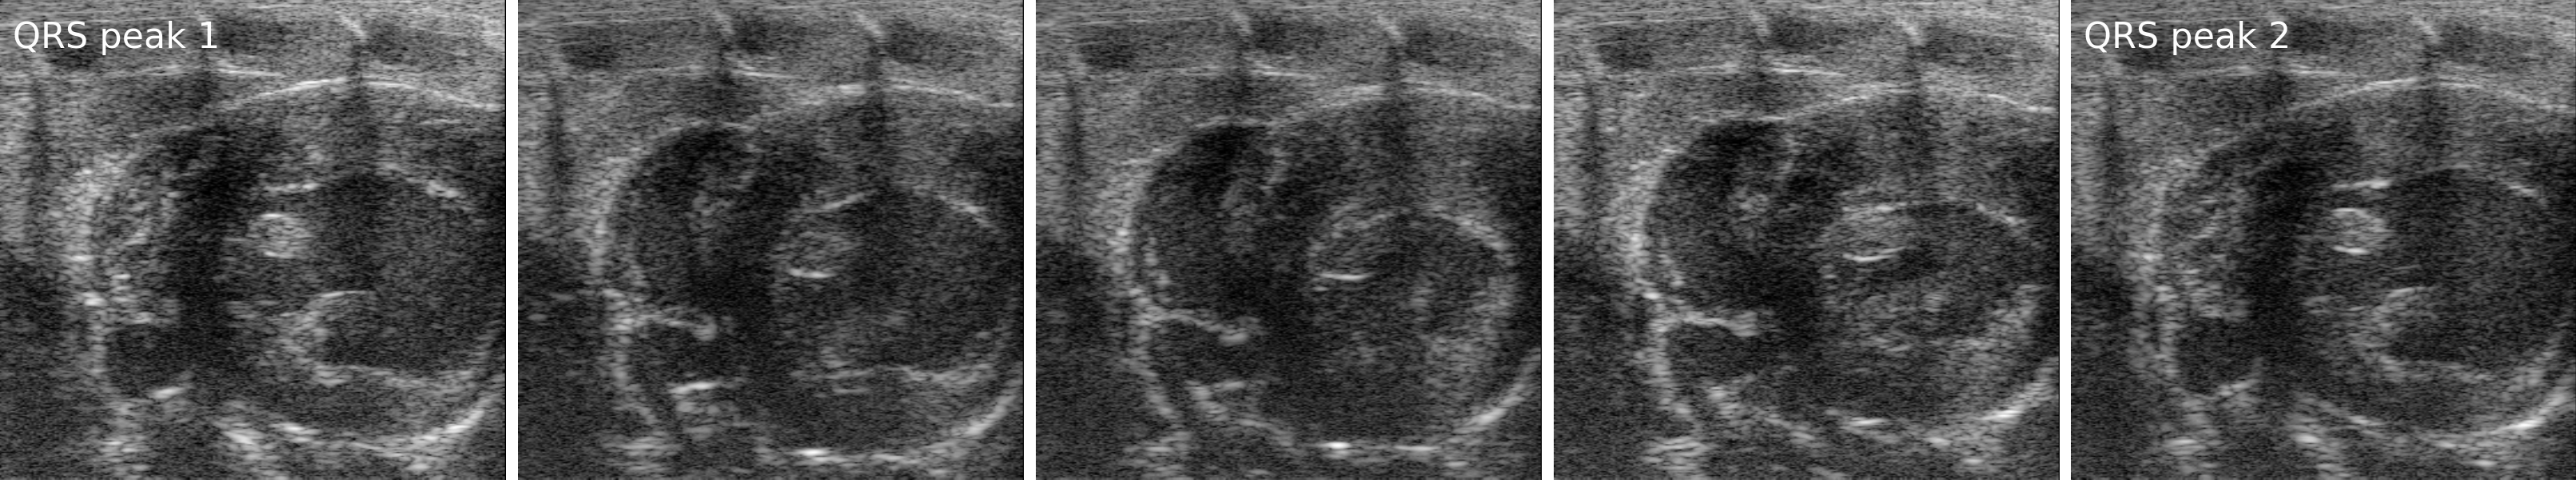
\includegraphics[width=4.25in]{figures/decoded/2015-07-27-10-36-06_2015-07-15-16-56-16_1.raw.bmode/qrs_peak_to_peak.png}\\
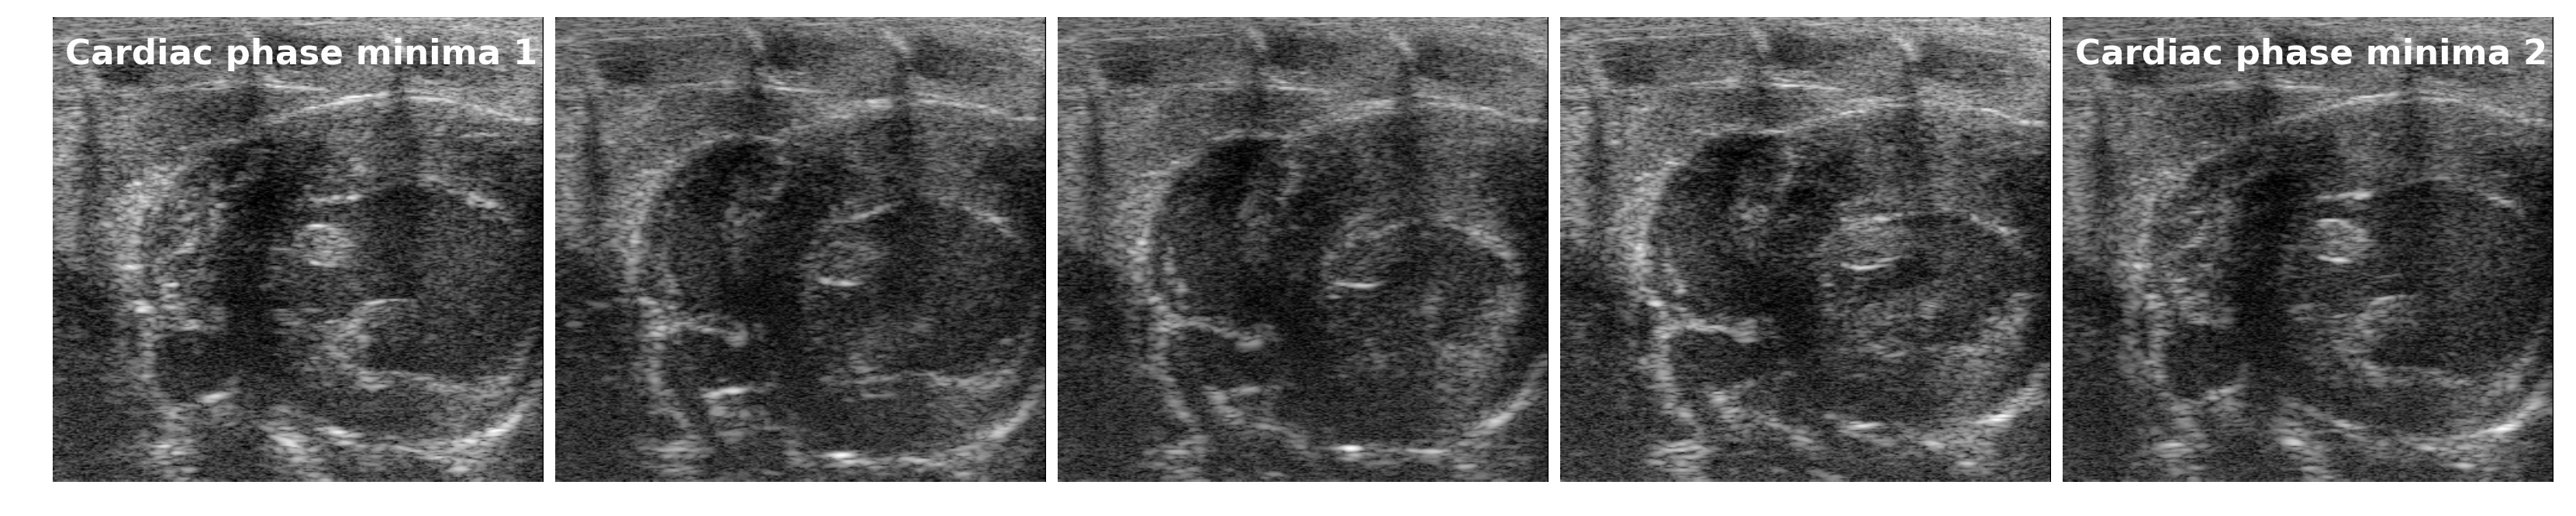
\includegraphics[width=4.25in]{figures/decoded/2015-07-27-10-36-06_2015-07-15-16-56-16_1.raw.bmode/instaphase_valley_to_valley.png}
\ionbox{4.25in}\\
%
\caption{Illustration of correspondence between ECG and the instantaneous cardiac phase estimated using our method: (a) ECG signal (blue) and the cardiac phase estimated using our method overlaid with peaks of the QRS complex (red circle) and the corresponding cardiac phase minima (black circle), (b) Five video frames evenly spaced in time between the first and second QRS peaks of the ECG signal (top-row) and the corresponding cardiac phase minima (bottom-row) constituting one cardiac cycle.}
\label{fig:instaphase_vs_ecg}
\end{IonFigT}
\vspace{-0.3cm}
\subsection{Estimation of instantaneous cardiac and respiratory phases}
\label{sec:method:phase_estimation}
%
\begin{IonFigT}
\centering
%
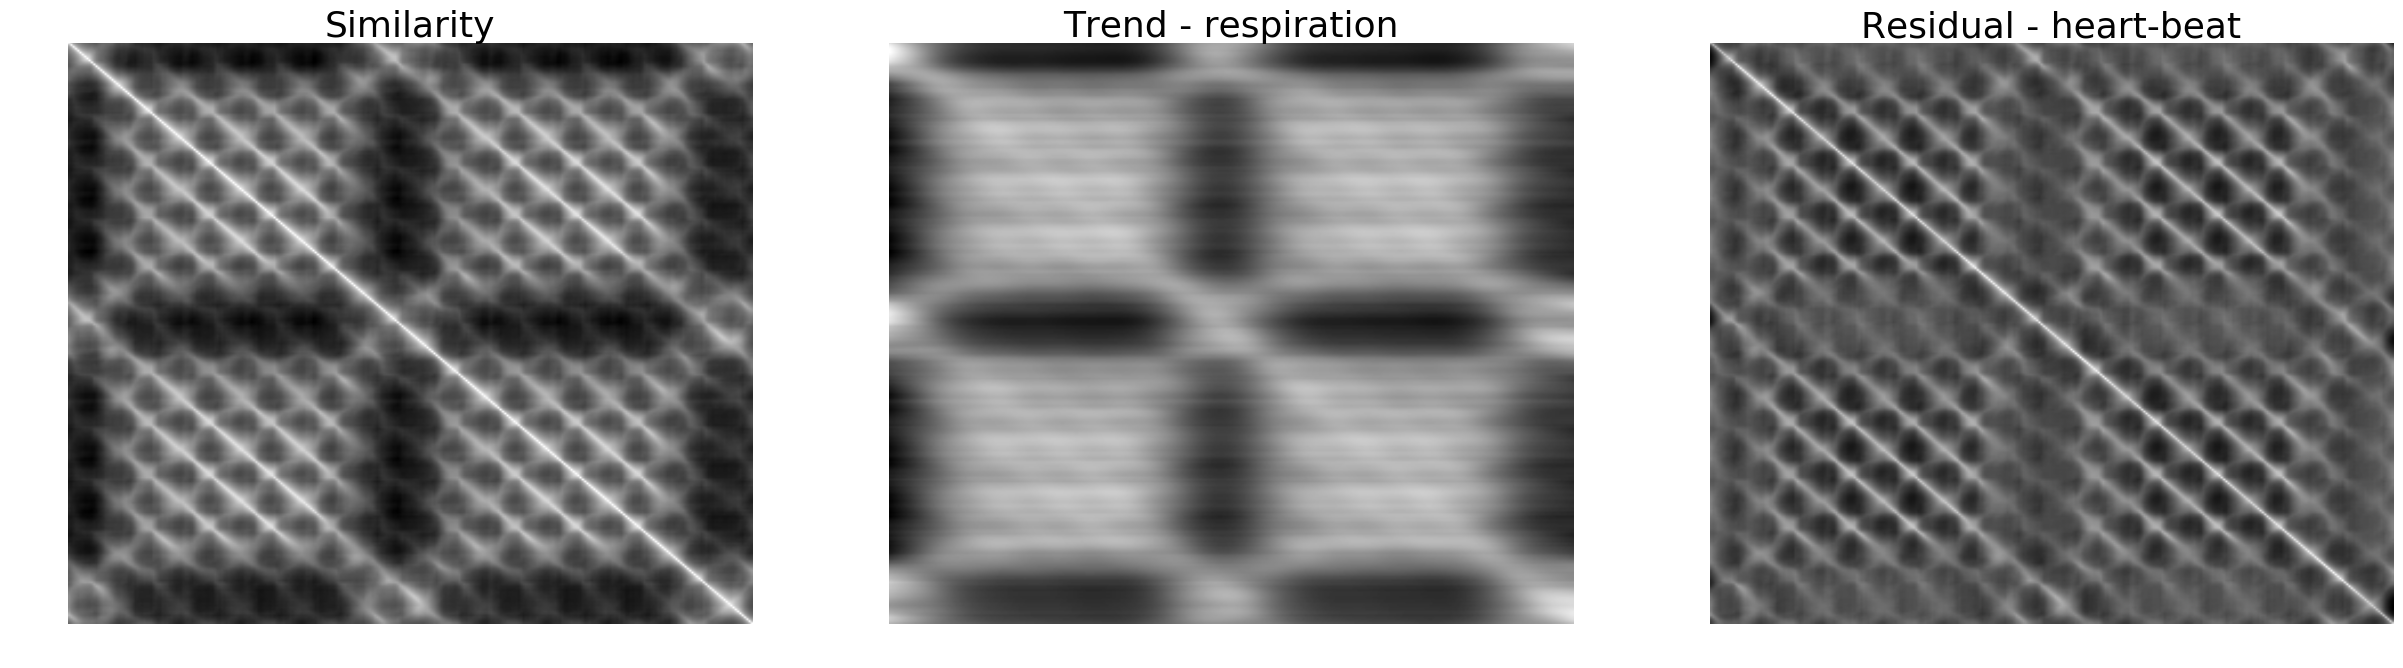
\includegraphics[width=3.9in]{figures/decoded/2015-07-27-10-36-06_2015-07-15-16-56-16_1.raw.bmode/simMat.png}
\ionbox{1.3in}\ionbox{1.3in}\ionbox{1.3in}\\
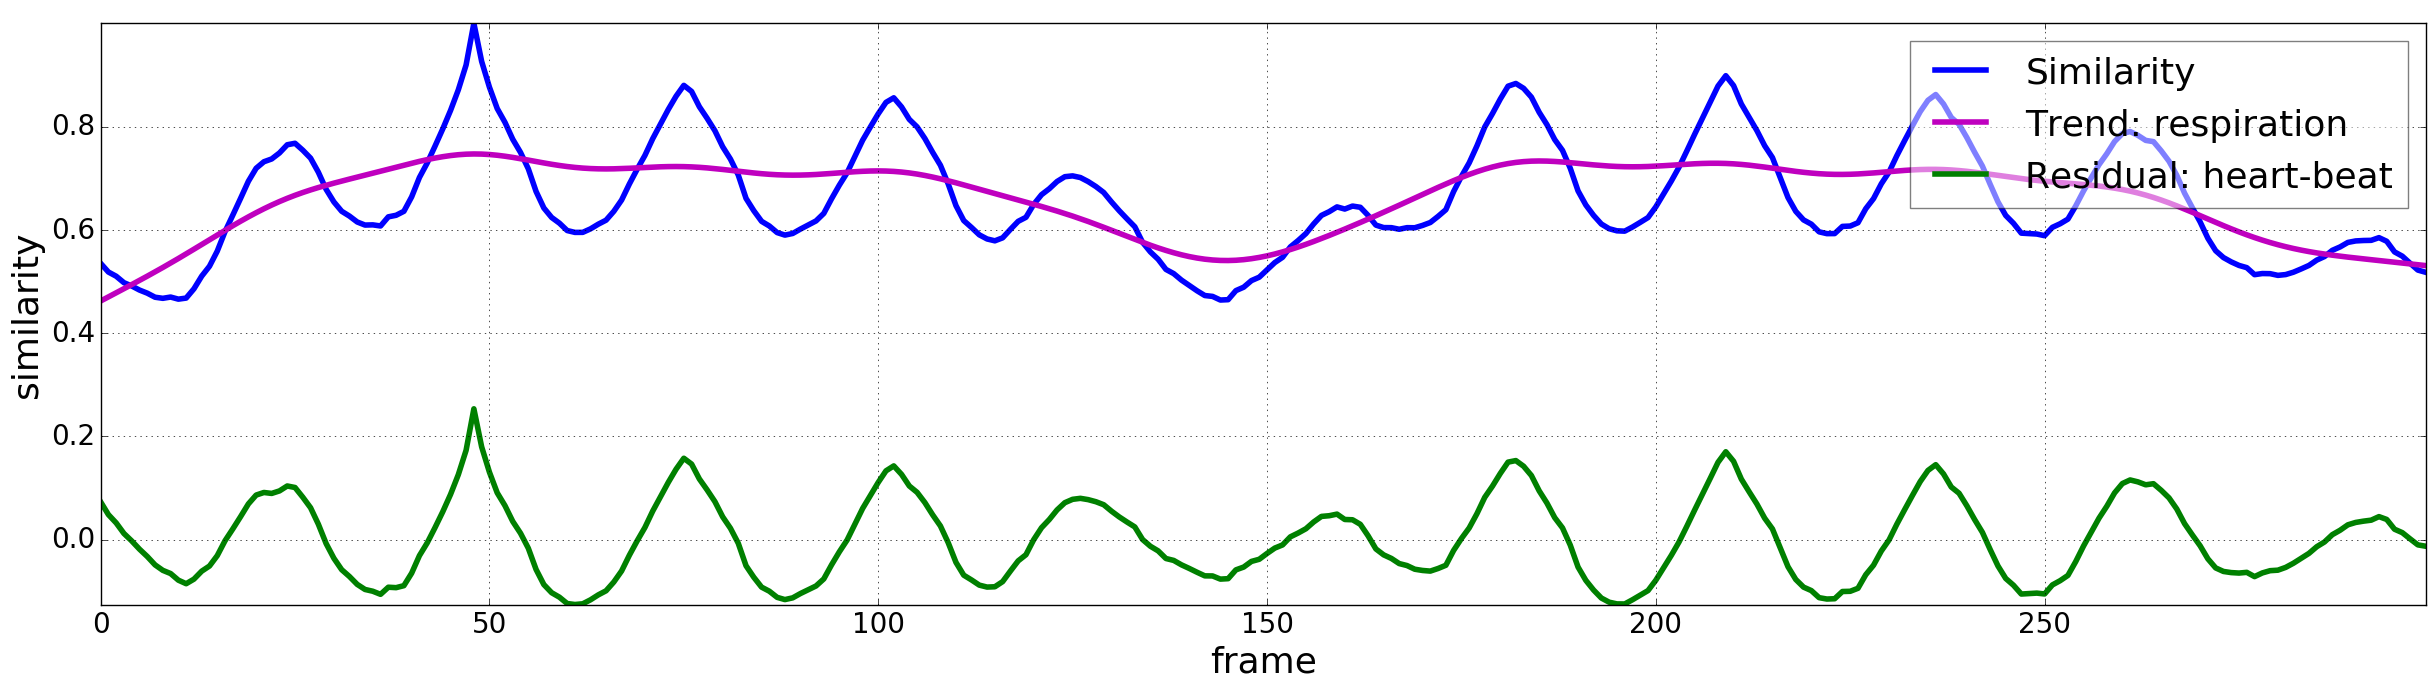
\includegraphics[width=4.25in]{figures/decoded/2015-07-27-10-36-06_2015-07-15-16-56-16_1.raw.bmode/season_trend_decomposition.png}
\ionbox{4.25in}\\
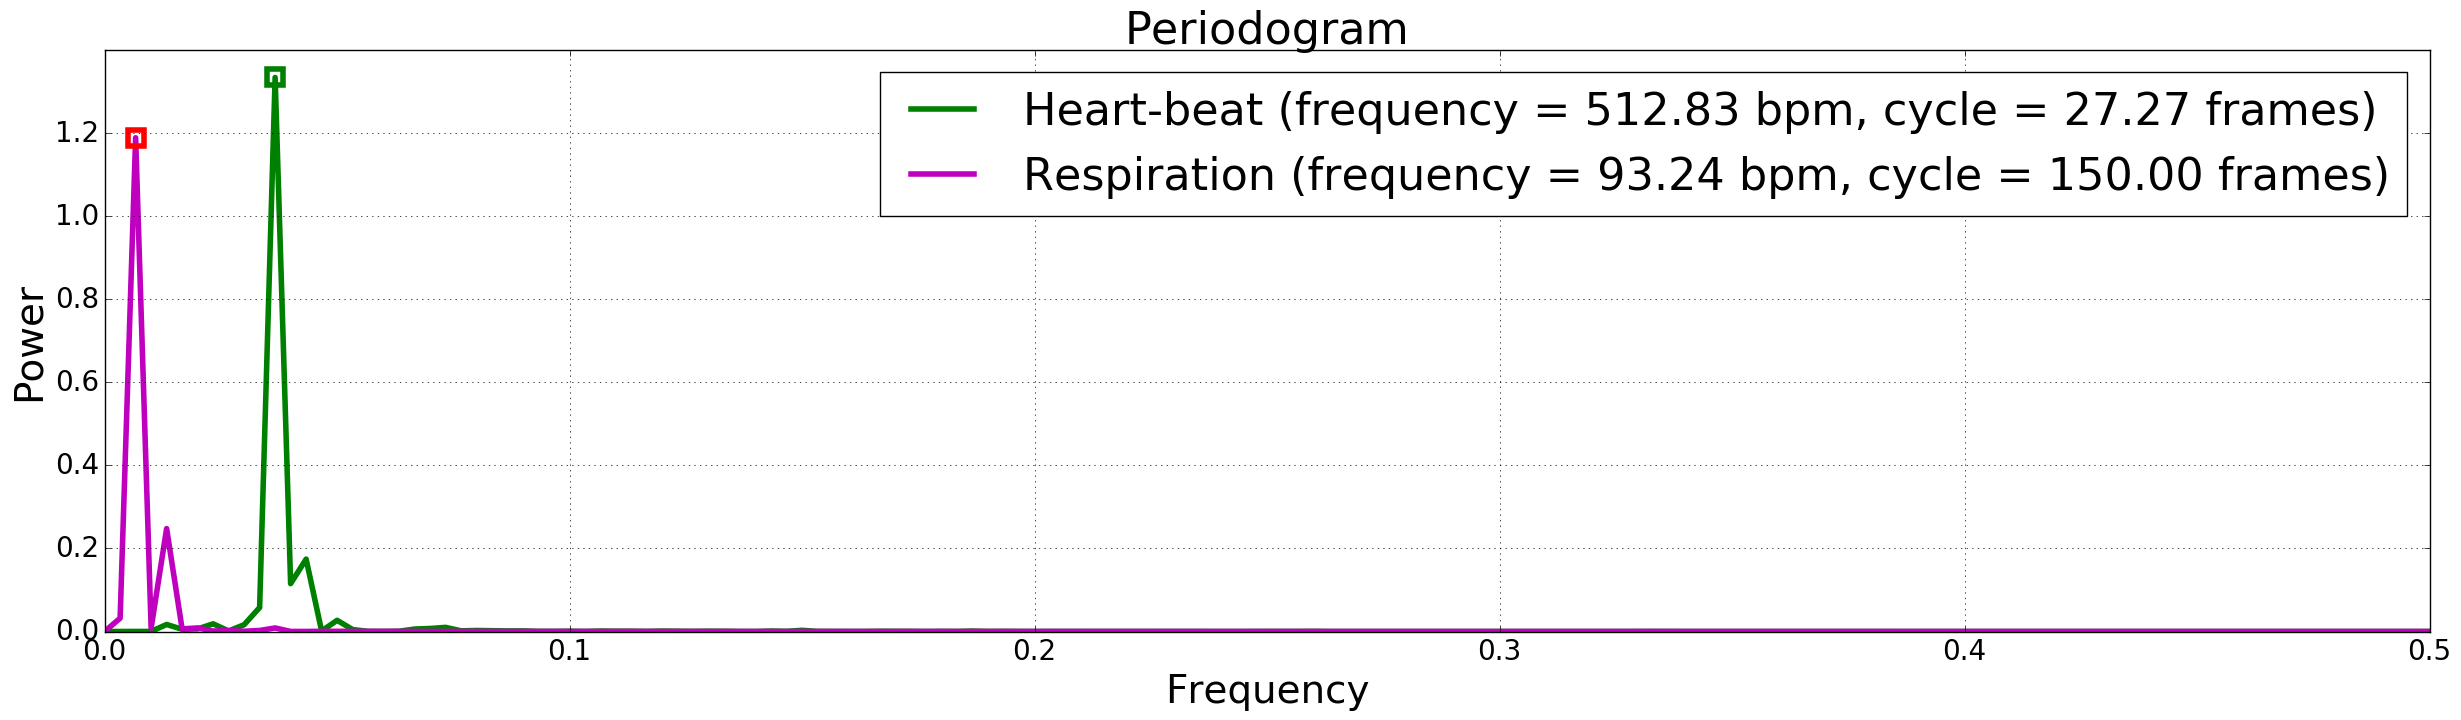
\includegraphics[width=4.25in]{figures/decoded/2015-07-27-10-36-06_2015-07-15-16-56-16_1.raw.bmode/periodogram.png}
\ionbox{4.25in}\\
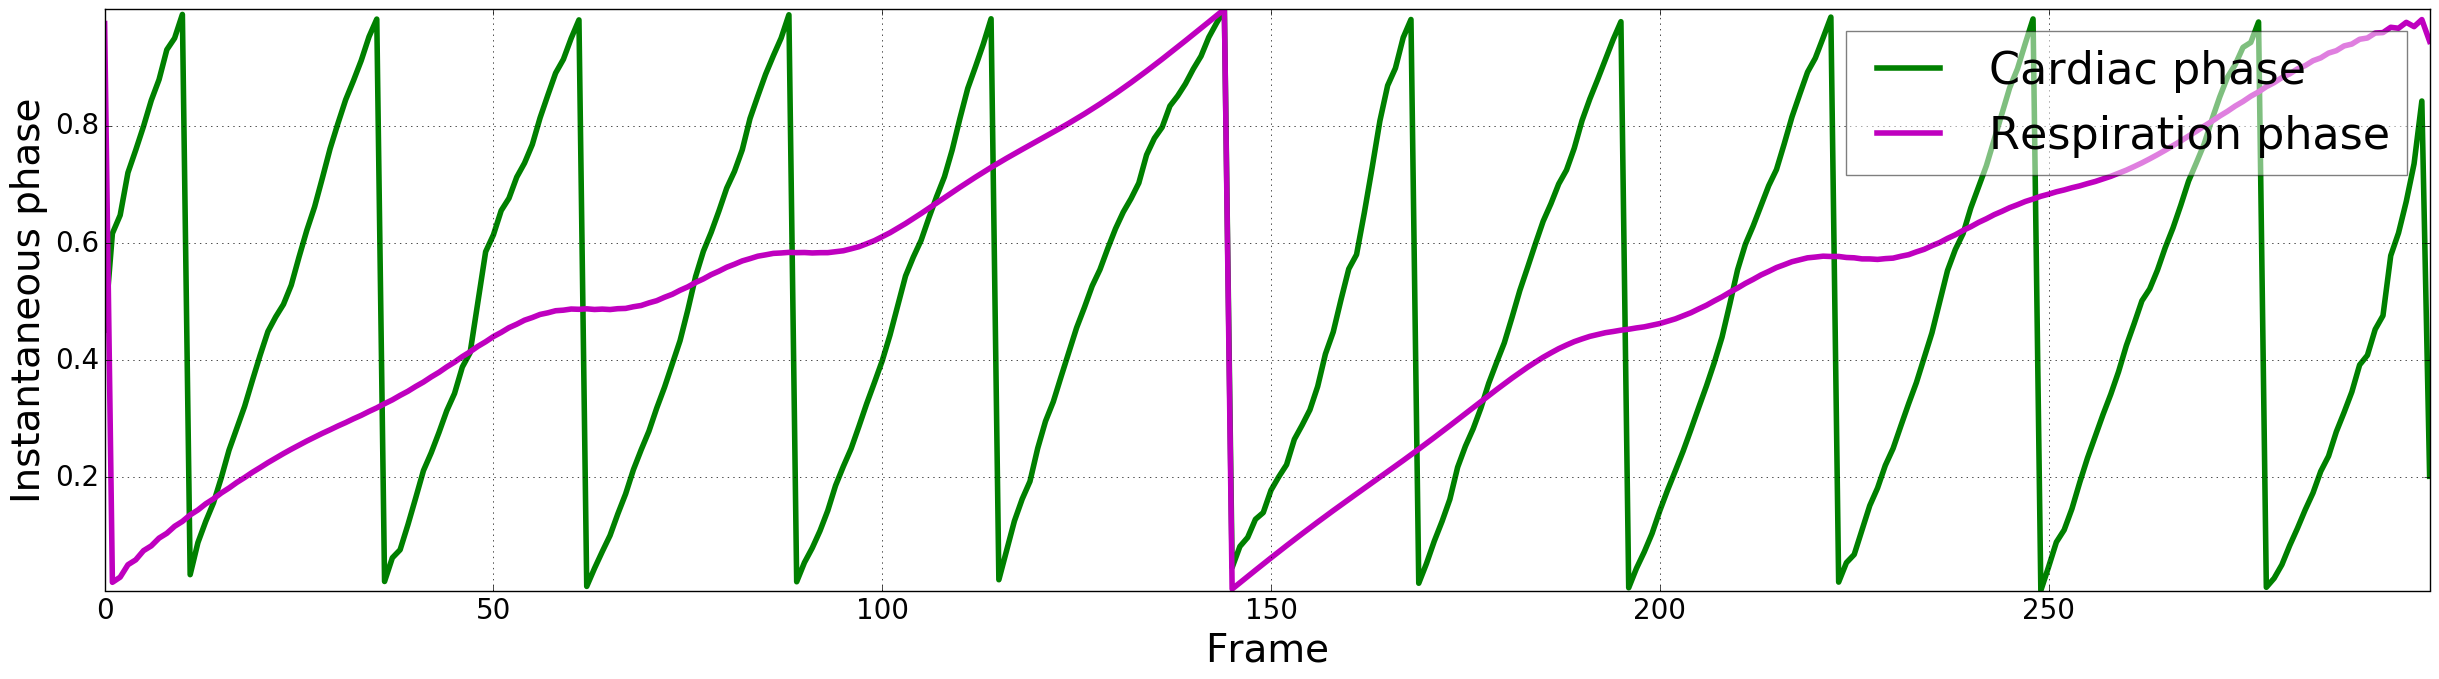
\includegraphics[width=4.25in]{figures/decoded/2015-07-27-10-36-06_2015-07-15-16-56-16_1.raw.bmode/instantaneous_phase.png}
\ionbox{4.25in}\\
%
\caption{Illustration of our phase estimation method: (a) Inter-frame similarity matrix, (b) Trend matrix corresponding to respiratory motion, (c) Residual matrix corresponding to beating heart motion, (d) Frame similarity $\hat{u}(t)$ selected for phase estimation with associated trend/respiration $\hat{\tau}_{resp}$ and residual/heart-beat $\hat{r}_{heart}$ signals, (e) Periodogram of heart-beat and respiration signals along with periodicity characteristics (e.g. frequency, cycle duration) calculated from the dominant frequency, and (f) Instantaneous cardiac and respiratory phases estimated using the Hilbert transform.}
\label{fig:phase_estimation}
\end{IonFigT}
%
While there have been numerous efforts for the estimation of instantaneous phase and/or frequency in periodic univariate time series data~\cite{Boashash1992}, there are not many methods that tackle this problem in a multivariate setting such as the case of cardiac ultrasound videos wherein thousands of variables (pixel intensities) are involved. Our strategy is to transform this complex multi-variate problem into a univariate one and take advantage of existing methods to solve the problem. 

	We first compute the similarity between all pairs of images/frames in the given periodic image sequence containing $N$ frames to create a symmetric matrix $A \in R^{N \times N}$ where in the element $A(i,j)$ is equal to the similarity between the $i^{th}$ and $j^{th}$ frame. Here in, we use normalized correlation (also known as the Pearson correlation coefficient) to quantify inter-frame similarity; but in principle, other image similarity metrics can be used. Each row in the inter-frame similarity matrix $A$ can now be seen as a univariate time series. If the similarity metric is chosen with care and if the corresponding frame is not significantly corrupted, this time series will preserve the periodicity characteristics of the original image sequence. Figure \ref{fig:phase_estimation}(a) shows the inter-frame similarity matrix of one of our cardiac ultrasound videos wherein the periodicity of low-frequency respiratory motion and high-frequency beating heart motion can observed. 

	Next, we use a trend extraction technique called the Hodrick-Prescott (HP) filter~\cite{Alexandrov2012} to decompose the frame similarity signal $u^i(t)$ corresponding to each row $i$ of the matrix $A$ into a sum of two components: (i) Trend component $\tau^i_{resp}(t)$ with periodicity characteristic of only respiratory motion, and (ii) Residual component $r^i_{heart}(t)$ with periodicity characteristic of only beating heart motion. The HP filter performs the decomposition of $u^i(t) = \tau^i_{resp}(t) + r^i_{heart}(t)$ by solving the following optimization problem:
\begin{equation}	
\argmin{\tau^i_{resp}(t)} \left[ \sum_{t=1}^{N}  \left(u^i(t) - \tau^i_{resp}(t) \right)^2  + \lambda \sum_{t=1}^{N-1} \left( \nabla^2 \tau^i_{resp}(t) \right)^2 \right] 
\end{equation}
where $\nabla^2\tau^i_{resp}(t) = \tau^i_{resp}(t+1) - 2 \tau^i_{resp}(t) + \tau^i_{resp}(t-1)$ is the second-order difference or derivative of the trend signal and $\lambda=6400$ is penalty parameter. Let $A_{resp}$ and $A_{heart}$ be the matrices whose rows contain the trend/respiratory and residual/heart-beat components (Figures~\ref{fig:phase_estimation}(b,c)), respectively, of the frame similarity signal in the corresponding rows of matrix $A$. We now need to select the signals corresponding to one of the rows for phase estimation. To minimize the effect of any noise, we pick the row for which the periodogram or power-frequency distribution of the heart-beat component in $A_{resp}$ has minimum entropy. Let $\hat{u}(t)$ be the selected frame similarity signal and let $\hat{\tau}_{resp}(t)$ and $\hat{r}_{heart}(t)$  be its associated trend and residual components  (Figure~\ref{fig:phase_estimation}(d)) that we will henceforth refer to as respiration and heart-beat signals, respectively.

	Next, considering the narrow-band nature of the respiration and heart-beat signals (see  Figure~\ref{fig:phase_estimation}(e)), we use the Hilbert transform~\cite{Boashash1992} to estimate the instantaneous phase of each frame. Specifically, we compute the instantaneous phase $\phi(t) \in \left [  -\pi, \pi\right )$ of a periodic time series $x(t)$ using its Hilbert transform $H_x(t)$ as follows: $\phi(t) = arctan \left( \frac{H_x(t)}{x(t)}\right)$ and map $\phi(t)$ from $\left [  -\pi, \pi\right )$ to $\left [  0, 1\right )$. Let $\hat{\phi}_{heart}(t)$ and $\hat{\phi}_{resp}(t)$ denote the instantaneous cardiac and respiratory phases (Figure~\ref{fig:phase_estimation}(f)) computed from the respiration and heart-beat signals, respectively.
%
\vspace{-0.3cm}
\subsection{Gating out respiratory frames}
\label{sec:method:gating}
%
%
\begin{IonFigT}
\centering
%
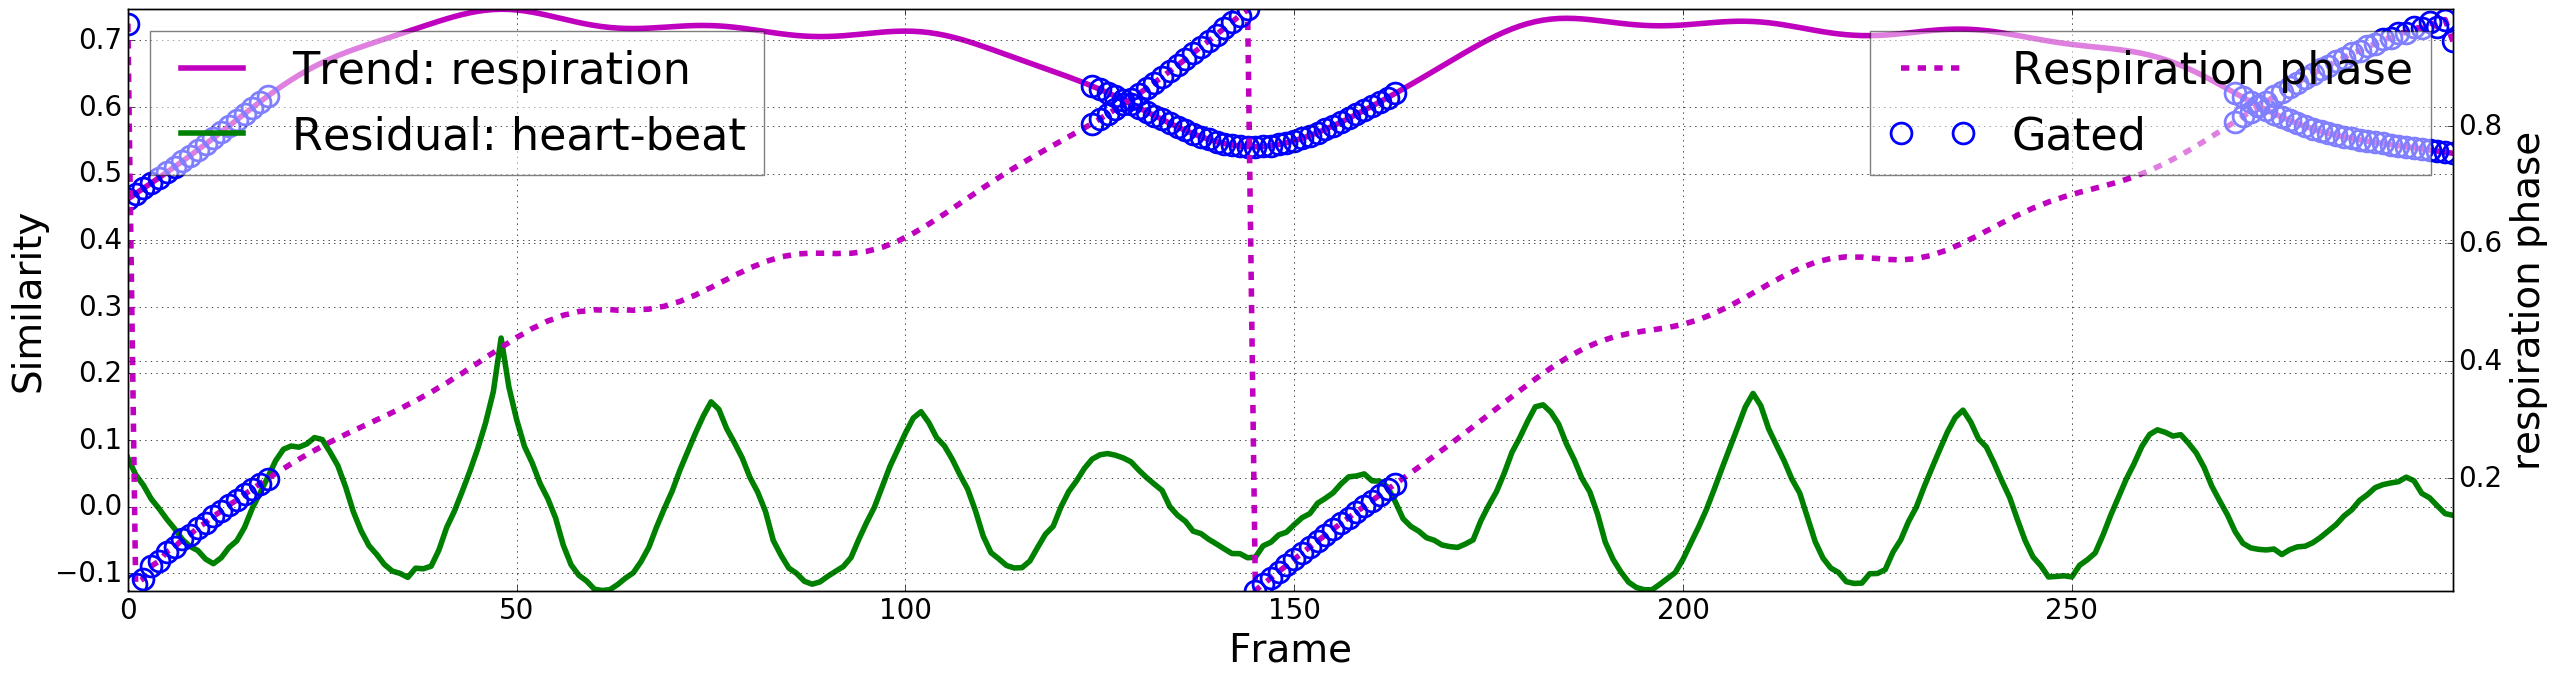
\includegraphics[width=4.25in]{figures/decoded/2015-07-27-10-36-06_2015-07-15-16-56-16_1.raw.bmode/respiratory_phase_gating.png}
\ionbox{4.25in}\\
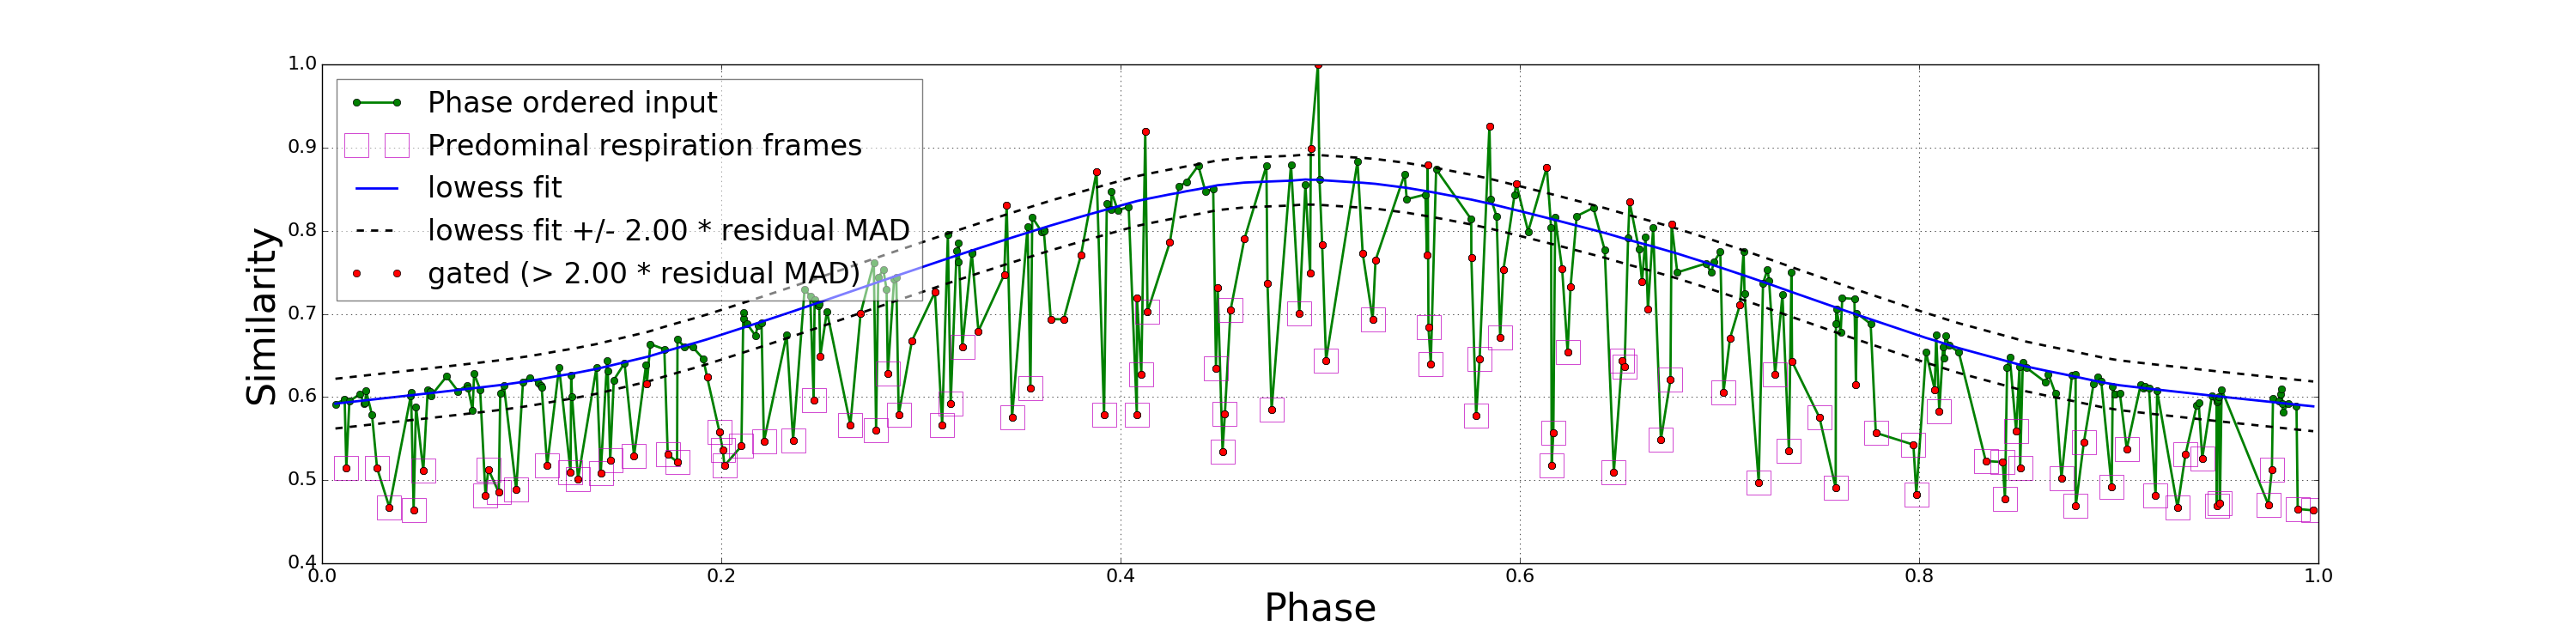
\includegraphics[width=4.25in]{figures/decoded/2015-07-27-10-36-06_2015-07-15-16-56-16_1.raw.bmode/robust_lowess_gating.png}
\ionbox{4.25in}\\
%
\caption{Illustration of the respiratory gating method: (a) Frames $F_{cutoff}$ discarded (blue circles) in step-1 overlaid with the respiration, heart-beat, and respiratory phase signals (b) heart-beat signal $\hat{r}_{heart}(t)$ vs cardiac phase $\hat{\phi}_{heart}(t)$ overlaid with frames $F_{cutoff}$ discarded in step-1 (blue circle), LOWESS fit $L(\phi)$ (black solid), upper and lower bounds or 95\% confidence interval $(L(\phi) \pm 2.0 * \hat{\sigma}_L)$ of non-respiratory frames (black dotted), and frames $F_{resp}$ (red circles) gated after step-2.}
\label{fig:respiratory_gating}
\end{IonFigT}
%
Once the cardiac and respiratory phases of each frame have been estimated, they can be used to select or filter out frames from a desired part/point in the periodic cycle, a process commonly referred to as gating. In this section, we present a robust two-step method that uses these phase estimates to filter out video frames with significant respiratory motion.

	In the first step, based on the observation that respiratory motion mainly occurs around the minima of the respiration signal $\hat{\tau}_{resp}(t)$ (pink curve in Fig.~\ref{fig:phase_estimation}(d)) with respiratory phase $\hat{\phi}_{resp}(t) = 0$, we perform a rough initial gating by discarding the frames $F_{cutoff} = \left \{ t \mid \hat{\phi}_{resp}(t) < c \vee \hat{\phi}_{resp}(t) > (1 - c) \right \}$ whose phase distance from $\hat{\phi}_{resp}(t) = 0$ is below a specified cutoff value $c=0.2$. Figure~\ref{fig:respiratory_gating}(a) shows the discarded frames $F_{cutoff}$ overlaid on the respiration $\hat{\tau}_{resp}(t)$, heart-beat  $\hat{r}_{heart}(t)$, and respiratory phase $\hat{\phi}_{resp}(t)$ signals.
	
	In the second step, we learn a robust mapping $L(\phi) : \left [  0, 1\right ) \to R$ from cardiac phase to the heart-beat component of the frame similarity signal by fitting a robust non-parametric regression model called Locally weighted regression (LOWESS)~\cite{Cleveland1988} to the dataset $\left \{ \left(\hat{\phi}_{heart}(t), \hat{r}_{heart}(t) \right) \mid \forall t \notin F_{cutoff}  \right \}$ containing the pair of the cardiac phase $\hat{\phi}_{heart}(t)$ and heart-beat signal $\hat{r}_{heart}(t)$  values of all frames that do not belong to the set of frames $F_{cutoff}$ discarded in the first step above. Next, we compute a robust estimate of the standard deviation $\hat{\sigma}_{L}$ of non-respiratory frames around the LOWESS fit based on the median absolute deviation between the LOWESS fit $L( \hat{\phi}_{heart}(t) )$ and heart-beat signal $\hat{r}_{heart}(t)$ for all frames. Lastly, we gate out all frames $F_{resp} = \left \{ t : \lvert \hat{r}_{heart}(t) - L( \hat{\phi}_{heart}(t) ) \rvert   > k \times \hat{\sigma}_{L}  \right \}$
whose heart-beat signal value deviates from the LOWESS fit by more than $k = 2.0$ (95\% confidence interval) times the standard deviation $\hat{\sigma}_{L}$ (Figure~\ref{fig:respiratory_gating}(b)).	
%
%
\begin{IonFigT}
\centering
%
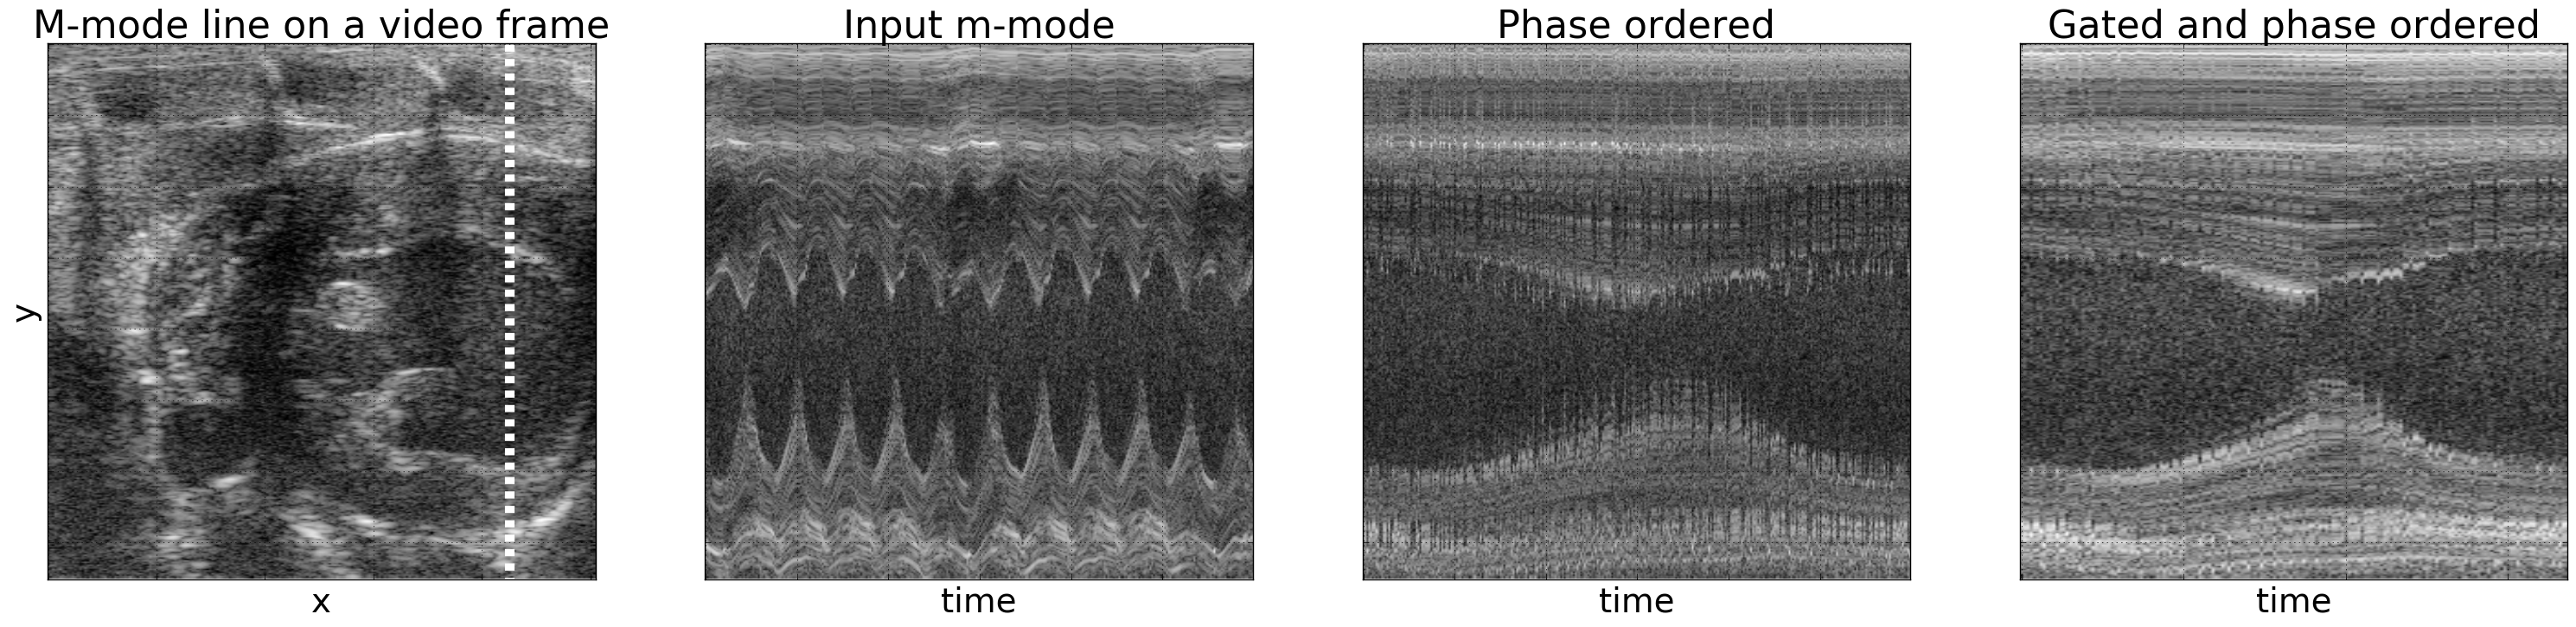
\includegraphics[width=4.5in]{figures/decoded/2015-07-27-10-36-06_2015-07-15-16-56-16_1.raw.bmode/phaseordered.png}
\ionbox{1.2in}\ionbox{1.1in}\ionbox{1.1in}\ionbox{1.1in}\\
%
\caption{Visualization of m-mode frames ordered by cardiac phase: (a) One of the frames in the video overlaid with the M-mode line shown in the next three images, (b) M-mode frames in the order they appear in the input video, (c) M-mode frames ordered by cardiac phase, and (d) Non-respiratory m-mode frames ordered by cardiac phase.}
\label{fig:phase_ordering}
\end{IonFigT}
%
\vspace{-0.3cm}
\subsection{Model to generate images by cardiac phase for super-resolution}
\label{sec:method:super_resolution}
%
In this section, we present a kernel regression model to reconstruct the image at any cardiac phase. This model can then be used to generate a single-cycle video representative of the subject's heart-beat at a higher temporal resolution.

Given a cardiac ultrasound video $I(t) : \{1, ..., N\} \to R^m$ of $N$ images with $m$ pixels each, we extract the heart-beat signal $\hat{r}_{heart}(t)$, estimate the instantaneous cardiac phase $\hat{\phi}_{heart}(t)$ of each frame, and compute the robust LOWESS fit $L(\phi) : \left [  0, 1\right ) \to R$ that maps cardiac phase to the heart-beat signal as described in Sections~\ref{sec:method:phase_estimation} and ~\ref{sec:method:gating}. We then use Nadarya-Watson (NW) kernel regression \cite{Bishop2006} to learn a function $M(\phi): [0, 1) \to R^m $ that reconstructs the image for any cardiac phase $\phi$ using a kernel-weighted local average as follows:
\begin{equation}
M(\phi) = \frac{\sum_{t = 1}^{N} K \left( \phi, \hat{\phi}_{heart}(t) \right) I(t)}{\sum_{t = 1}^{n} K \left( \phi, \hat{\phi}_{heart}(t) \right)} 
\end{equation}
where kernel $K\left( \phi, \hat{\phi}_{heart}(t) \right) = exp\left \{ -\frac{ \mid \phi - \hat{\phi}_{heart}(t) \mid^2}{2  \sigma^2_\phi} \right \} \times exp\left \{ -\frac{ \mid L(\phi) - \hat{r}_{heart}(t) \mid^2}{2  \sigma^2_{L}} \right \}$ is defined as the product of two radial-basis function (RBF) kernels. The first RBF kernel  weighs images inversely proportional to their distance (accounting for periodicity) in the cardiac phase space. Its bandwidth $\sigma_\phi$ is set equal to a constant $k_\phi = 0.4$ times the median difference in cardiac phase between consecutive frames of the given image sequence. The second RBF kernel weighs images inversely proportional to the deviation of their residual/heart-beat signal value from the LOWESS prediction $L(\phi)$. Its bandwidth $\sigma_{L}$ is set equal to a constant $k_L = 2.0$ times the robust estimate of standard deviation $\hat{\sigma}_{L}$ of non-respiratory frames ($\forall t \notin F_{resp}$) around the LOWESS fit. The function $M(\phi)$ can now be used to reconstruct a single-cycle video representative of the subject's heart-beat at any desired resolution/sampling of phase in the range $[0, 1)$. 
%
\vspace{-0.3cm}
\section{Experiments and Results}
\label{sec:results}
\vspace{-0.3cm}
%
We use cardiac ultrasound videos and associated ECG recordings of 6 mice to validate our methods. The ultrasound videos were acquired using the VisualSonics Vevo 2100 scanner at 233 frames per second. Each video consists of approximately 300 frames, 11 cardiac cycles, and 2 respiratory cycles.

	We validate the cardiac phase estimates of our method by comparing them with the ECG signal which is the gold standard for cardiac gating. Figure~\ref{fig:instaphase_vs_ecg}(a) shows a comparison between the ECG signal and the estimated cardiac phase signal for one of the 6 videos. Notice how well the locations of the QRS peaks in the ECG signal and the corresponding minima of the cardiac phase signal in each cycle match. Table 1 reports the $R^2$ correlation and the $mean \pm std$ error between the locations of the QRS peaks and the corresponding minima of the cardiac phase signals for all 6 videos. Figure~\ref{fig:instaphase_vs_ecg}(b) presents a visual comparison of five video frames evenly spaced in time between two consecutive QRS peaks (top-row) and corresponding minima of the cardiac phase signal (bottom-row). Figure~\ref{fig:phase_ordering} shows frames of an m-mode line through the ventricle before and after ordering by cardiac phase. The supplementary material includes a video showing the cardiac and respiratory phases of each frame for one of our datasets.
	
	We validate the accuracy of our kernel regression model for reconstructing images at any cardiac phase using leave-one-out-cross-validation (LOOCV). In each round of cross-validation, we randomly exclude one of the non-respiratory frames in the video, fit our kernel-regression model on the remaining frames, use the fitted model to reconstruct the image at the cardiac phase of the excluded frame, and compute the similarity between the reconstructed and original image using normalized correlation. The second column of Table~\ref{table:image_reconstruction} shows the $mean \pm std$ of normalized correlation between the reconstructed and the original images over 50 rounds of LOCCV for all 6 videos. As a \emph{baseline}, the third column of  Table~\ref{table:image_reconstruction} shows the $mean \pm std$ of the normalized correlation between frames at QRS peaks of the ECG signal. The supplementary material includes single-cycle videos at 2x and 4x temporal resolution generated using the kernel regression model wherein the motion of heart chambers and valves is much clear than the original video. 
%
%
\begin{table}[t]
\begin{small}
\begin{minipage}[t]{0.45\linewidth}
\centering
\caption{Match between frame positions of QRS peaks in ECG signal and corresponding cardiac phase minima.}
%\vspace{-0.1cm}
\begin{tabular}{|c|c|c|}
\hline
\multicolumn{1}{|l|}{} & \multicolumn{2}{l|}{QRS peak frame identification} \\ \hline
VID & $R^2$ & $mean \pm std \; error$ \\ \hline
1 & \; 0.9995 \; & 1.55 $\pm$ 0.89 \\ \hline
2 & \; 0.9995 \; & 1.36 $\pm$ 1.15 \\ \hline
3 & \; 0.9996 \; & 1.45 $\pm$ 0.89 \\ \hline
4 & \; 0.9998 \; & 0.73 $\pm$ 0.62 \\ \hline
5 & \; 0.9990 \; & 2.09 $\pm$ 1.78 \\ \hline
6 & \; 0.9992 \; & 1.40 $\pm$ 1.74 \\ \hline
\end{tabular}
\label{table:phase_estimation}
\end{minipage}
%
\hspace{0.5cm}
%
\begin{minipage}[t]{0.45\linewidth}
\centering
\caption{Evaluation of our kernel regression model. Leave one out cross-validation (LOOCV) of 50 rounds.}
%\vspace{-0.1cm}
\begin{tabular}{|c|c|c|}
\hline
\begin{tabular}[c]{@{}c@{}}VID \\ $\;$ \end{tabular} & \begin{tabular}[c]{@{}c@{}}LOOCV (50)\\ $mean \pm std \; ncorr$\end{tabular} & \begin{tabular}[c]{@{}c@{}}QRS Peak Frames\\ $mean \pm std \; ncorr$\end{tabular} \\ \hline
1 & 0.8562 $\pm$ 0.0366 & 0.7981 $\pm$ 0.0532 \\ \hline
2 & 0.8558 $\pm$ 0.0525 & 0.7877 $\pm$ 0.0503 \\ \hline
3 & 0.8592 $\pm$ 0.0348 & 0.7849 $\pm$ 0.0457 \\ \hline
4 & 0.8713 $\pm$ 0.0348 & 0.8395 $\pm$ 0.0486 \\ \hline
5 & 0.8655 $\pm$ 0.0312 & 0.8196 $\pm$ 0.0476 \\ \hline
6 & 0.8736 $\pm$ 0.0278 & 0.8270 $\pm$ 0.0778 \\ \hline
\end{tabular}
\label{table:image_reconstruction}
\end{minipage}
\vspace{-0.5cm}
\end{small}
\end{table}
%
%
\vspace{-0.5cm}
\section{Conclusion}
\label{sec:conclusion}
\vspace{-0.2cm}
%
In this paper, we have presented a novel method to estimate the instantaneous cardiac and respiratory phases directly from the cardiac ultrasound video, thereby eliminating the need of additional hardware to monitor them in, for example, small animal studies. We have also presented a robust non-parametric regression technique for gating out respiratory frames and a novel kernel regression model for reconstructing images at any cardiac phase to facilitate temporal super-resolution. We next plan to evaluate our methods on more datasets and address remaining pitfalls. Our phase estimation method makes a strong assumption of periodicity which may not hold in the case of subjects with cardiac arrhythmia. To address this, we will look into univariate methods for phase estimation in quasi-periodic signals that are less susceptible noise. The use of normalized correlation to measure inter-frame similarity relies on an inherent assumption that a large part of the image is pulsating. To relax this, we will devise local patch-based similarity measures. Lastly, the local weighted average used by our NW kernel regression model may cause blurring at high temporal magnification. We plan to alleviate this using manifold kernel regression~\cite{Davis2010} that computes the weighted average in a diffeomorphic registration sense.
%
\vspace{-0.2cm}
%
\bibliographystyle{splncs03}
\bibliography{library}
\end{document}







